\chapter{Título del Capítulo 2}
\label{chapter:dos}

\noindent Los capítulos intermedios servían para cubrir los siguientes aspectos: antecedentes, problemática o estado del arte, objetivos, fases y desarrollo del proyecto.

En el capítulo anterior se ha introducido bla, bla, bla de la \autoref{fig:other}, bla....

\section{Primera sección de otro capítulo}

\begin{figure}[htb]
   \centering
   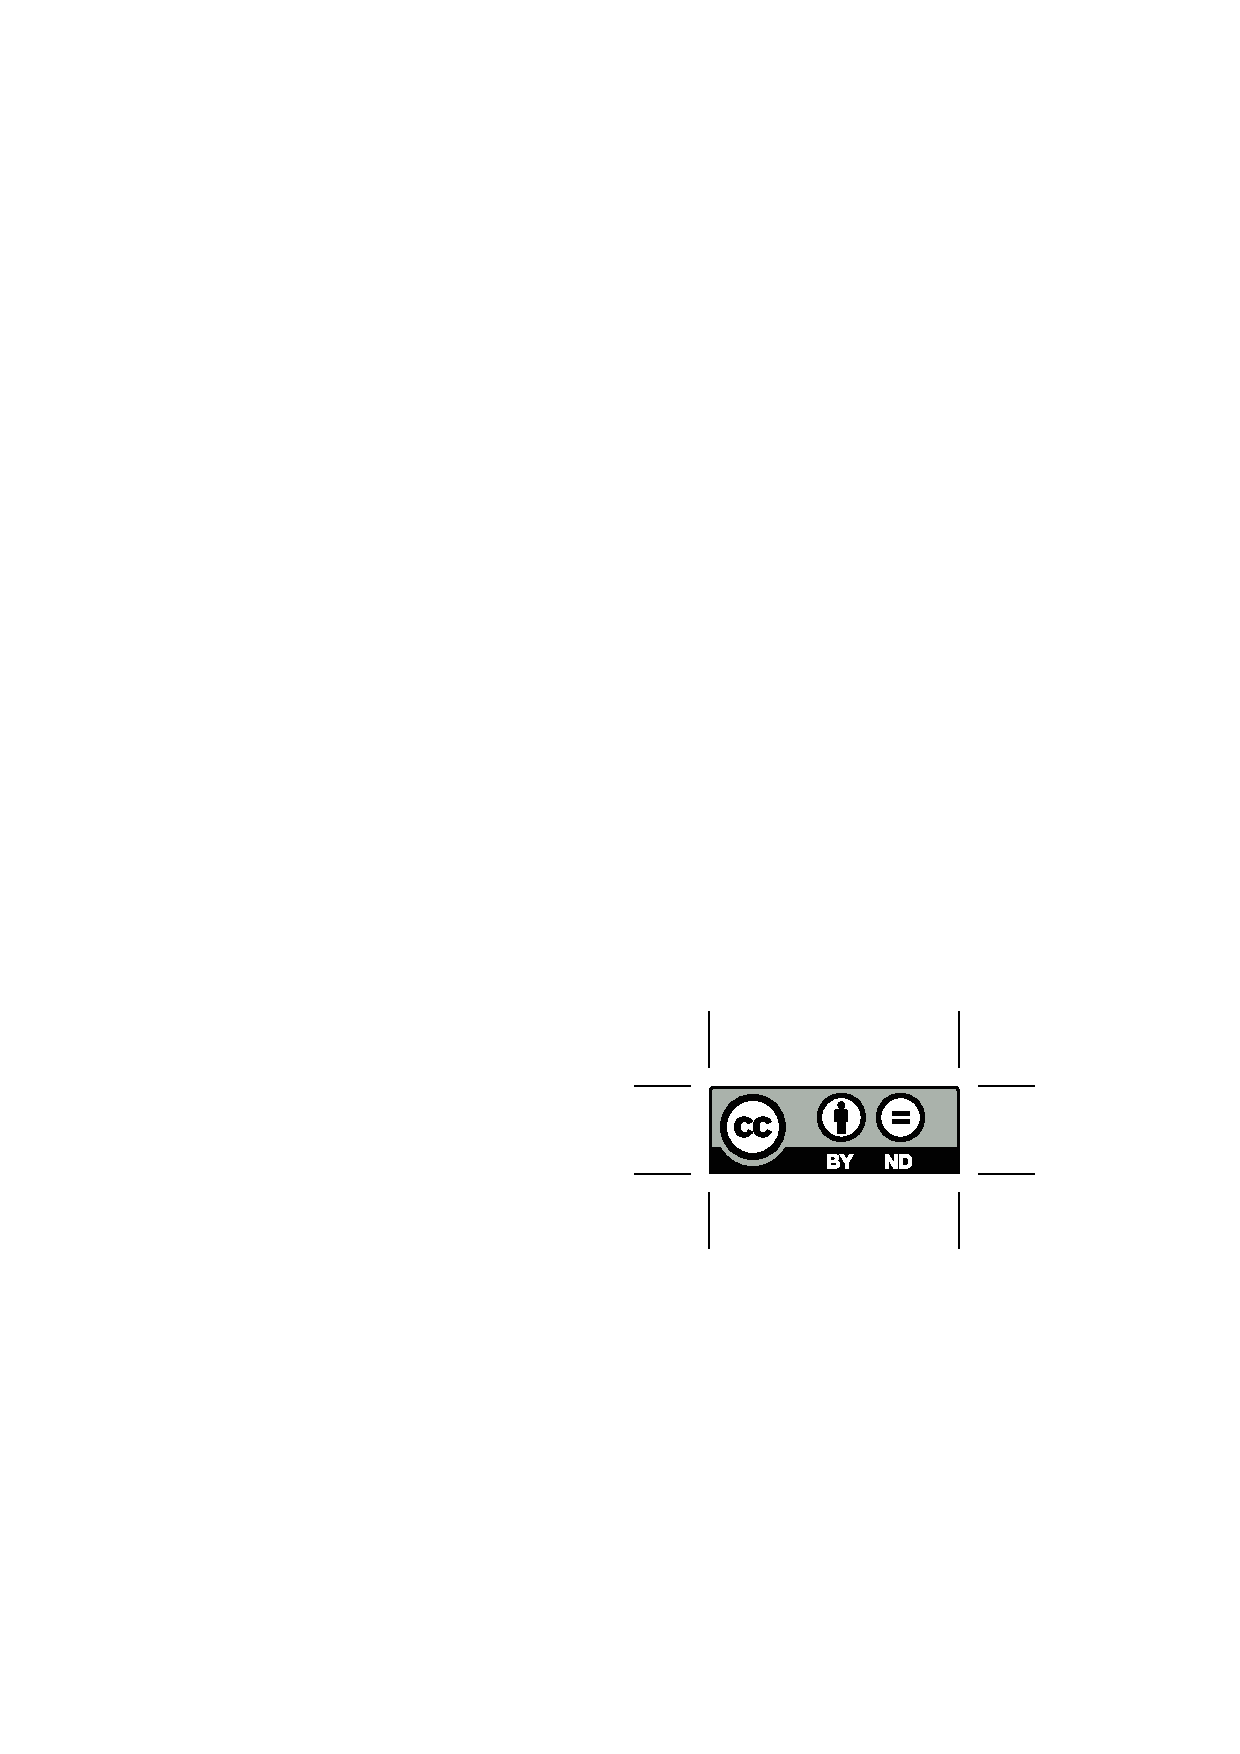
\includegraphics[width=0.5\linewidth]{images/licenses/by-nd}
   \caption{Otra figura.}
   \label{fig:other}
\end{figure}

\section{Segunda sección de otro capítulo}

También se pueden citar artículos\parencite{examplearticle}, libros o repositorios de \cite{examplegithub}.